\documentclass[11pt]{article}
\usepackage[utf8]{inputenc}
\usepackage{geometry}
\usepackage{amsmath}
\usepackage{amsfonts}
\usepackage{amssymb}
\usepackage{graphicx}
\usepackage{listings}
\lstdefinelanguage{CSS}{
    keywords={
        color,
        background,
        background-color,
        font,
        font-family,
        font-size,
        font-weight,
        width,
        height,
        margin,
        padding,
        border,
        border-radius,
        display,
        position,
        top,
        right,
        bottom,
        left,
        flex,
        flex-direction,
        justify-content,
        align-items,
        grid,
        gap,
        overflow,
        text-align,
        line-height,
        opacity,
        cursor,
        transition,
        transform,
        box-shadow
    },
    sensitive=true,
    comment=[l]{//},
    morecomment=[s]{/*}{*/},
    morestring=[b]",
    morestring=[b]'
}
\lstdefinelanguage{JavaScript}{
    keywords={
        break, case, catch, class, const, continue, debugger, default,
        delete, do, else, export, extends, finally, for, function,
        if, import, in, instanceof, let, new, return, switch, this,
        throw, try, typeof, var, void, while, with, yield, async, await
    },
    sensitive=true,
    comment=[l]{//},
    morecomment=[s]{/*}{*/},
    morestring=[b]",
    morestring=[b]'
}
\lstdefinelanguage{Python}{
    keywords={
        and, as, assert, async, await, break, case, class, continue,
        def, del, elif, else, except, finally, for, from, global,
        if, import, in, is, lambda, match, nonlocal, not, or, pass,
        raise, return, try, while, with, yield, True, False, None
    },
    sensitive=true,
    comment=[l]{\#},
    morestring=[b]",
    morestring=[b]'
}
\usepackage{xcolor}
\usepackage[colorlinks=true, 
            urlcolor=blue, 
            citecolor=blue, 
            linkcolor=blue]{hyperref}
\providecommand*{\listingautorefname}{Listing}
\usepackage{booktabs}
\usepackage{textcomp}
\usepackage{fancyhdr}
\usepackage{tabularx}
\usepackage{enumitem}
\usepackage{caption}
\captionsetup{
    labelfont=bf,
    textfont=normalfont
}
\usepackage{float} % in preamble

\usepackage{tikz}
\usetikzlibrary{positioning,arrows.meta}

\setlength{\parindent}{0pt}

% ------------------------------------------------

\geometry{margin=1in}

\pagestyle{fancy}
\fancyhf{}
\fancyhead[L]{\normalsize \textbf{Group 4: Light Intensity Monitoring}} 
\fancyhead[R]{
\includegraphics[height=1.2cm]{Figures/logo.png}} 
\fancyfoot[C]{\thepage}

\setlength{\headheight}{28pt} % needed for logo


\lstset{
    basicstyle=\ttfamily\footnotesize,
    numbers=left,
    numberstyle=\tiny,
    numbersep=8pt,
    frame=single,
    breaklines=true,
    showstringspaces=false,
    tabsize=4,
    commentstyle=\color{green!50!black},
    keywordstyle=\color{blue},
    stringstyle=\color{red}
}

% ------------------------------------------------

\begin{document}

% --- Custom Title Block ---
\begin{center}
    
\includegraphics[width=0.7\textwidth]{Figures/logo.png}\\[2cm]

    {\Huge
    \textbf{Computer Network Group Project}\\[1cm]

    \textbf{Real-Time Light Intensity Monitoring}\\[0.1cm]
    \textbf{System Using STM32 with}\\[0.3cm]
    \textbf{Web-Based Interface}
    }\\[1cm]
    
    {\huge July 21, 2026}
\end{center}

\thispagestyle{empty}   % First page: no header or footer

\vspace{0.5cm}
\begin{center}
{\LARGE Group 4:}

\vspace{0.5em}

\renewcommand{\arraystretch}{2}
\begin{tabular}{ll}
{\LARGE Bui Thanh Vinh} & {\LARGE 102240486} \\
{\LARGE Nguyen Quang Nhat} & {\LARGE 102240051} \\
{\LARGE Dinh Quoc Hung} & {\LARGE 102240117} \\
{\LARGE Nguyen Minh Huy} & {\LARGE 102240118} \\
\end{tabular}
\end{center}


\vfill  % Push everything else (like TOC) to bottom
\begin{flushright}
\normalsize
\textbf{Module:} Computer Network (SS25/26)\\[0.5cm]
\textbf{Professor:} Prof. Dr.-Ing. Ansgar Meroth
\end{flushright}


\newpage
\tableofcontents
\newpage

% ------------------------------------------------
\section{Introduction}

The Internet of Things (IoT) has become an essential technology for monitoring and controlling physical environments through interconnected devices. In many IoT applications, sensor data must be acquired, transmitted, processed, and visualized in real time to provide users with immediate information about the monitored system. Developing a reliable end-to-end communication pipeline between embedded hardware and a graphical user interface is therefore an important aspect of modern embedded system design.\\[0.1em]

This project presents the implementation of a real-time light intensity monitoring system using a BH1750 digital light sensor and an STM32 microcontroller. The BH1750 sensor continuously measures ambient illumination, while the STM32 acquires the sensor data through the Inter-Integrated Circuit (I\textsuperscript{2}C) communication protocol. The measured values are transmitted to a personal computer through a Universal Serial Bus (USB) Virtual COM Port.\\[0.1em]

On the software side, a Python application reads the incoming serial data, validates the received measurements, and converts them into JavaScript Object Notation (JSON) format. The JSON messages are then transmitted to a Node.js backend through a WebSocket connection. The backend server broadcasts the sensor data to one or more connected web clients, allowing multiple users to observe the sensor measurements simultaneously. Finally, a browser-based graphical user interface (GUI) displays the received illumination values and visualizes the data in real time using an interactive graph.\\[0.1em]

The objective of this project is to design and implement a complete data acquisition and visualization pipeline, beginning with physical sensing and ending with real-time presentation on a web interface. The system demonstrates the integration of embedded programming, serial communication, WebSocket networking, and web technologies to provide an efficient and scalable IoT monitoring solution.


% ------------------------------------------------
\section{Sensor Description and Technical Background}

This section introduces the hardware components used in the proposed monitoring system. The BH1750 digital light sensor is responsible for measuring ambient illumination, while the STM32 microcontroller acquires the sensor data through the I\textsuperscript{2}C communication interface and forwards the measurements to the host computer via USB Virtual COM Port. The technical characteristics and operating principles of both components are described in the following subsections.

% ------------------------------------------------------------------------------------
\subsection{BH1750 Digital Light Sensor}

The BH1750 is a digital ambient light sensor developed by ROHM Semiconductor for measuring visible light intensity. Unlike analog photoresistors, the BH1750 integrates a photodiode, signal conditioning circuitry, a 16-bit analog-to-digital converter (ADC), and an I\textsuperscript{2}C communication interface into a single integrated circuit. As a result, the sensor directly outputs calibrated digital measurements, eliminating the need for external analog-to-digital conversion.\\[0.1em]

The sensor measures illumination in units of lux (lx), where one lux corresponds to one lumen per square meter. The measured digital value is converted into illumination using the relationship provided in the manufacturer datasheet \cite{bh1750_datasheet}

\begin{equation}
\text{Lux} = \frac{\text{Raw Output}}{1.2}.
\label{eq:lux_conversion}
\end{equation}

In this project, the BH1750 operates in Continuous High Resolution Mode, allowing continuous measurements with a resolution of approximately 1 lux while automatically updating the measurement register. The STM32 periodically reads the two-byte measurement result through the I\textsuperscript{2}C interface every second.\\[0.1em]

The BH1750 offers several advantages for embedded monitoring applications, including low power consumption, factory calibration, high measurement accuracy, and a simple two-wire communication interface. These characteristics make it well suited for real-time environmental monitoring systems.

\begin{figure}[H]
    \centering
    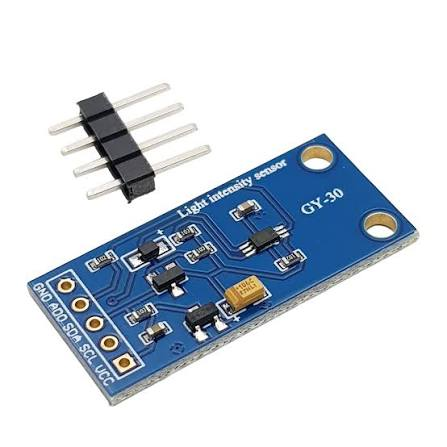
\includegraphics[width=0.45\textwidth]{Figures/BH1750.png}
    \caption{BH1750 digital ambient light sensor module.}
    \label{fig:bh1750}
\end{figure}


% ------------------------------------------------------------------------------------
\subsection{STM32 Microcontroller}

The embedded controller used in this project is an STM32 microcontroller from STMicroelectronics \cite{stm32_rm}. The microcontroller is responsible for configuring the BH1750 sensor, acquiring illumination measurements through the I\textsuperscript{2}C peripheral, and transmitting the measured data to a personal computer through a USB Virtual COM Port (USB CDC).\\[0.1em]

The firmware was developed using STM32CubeIDE together with the STM32 Hardware Abstraction Layer (HAL). After system initialization, the firmware configures the BH1750 for continuous high-resolution measurements. During each sampling cycle, two bytes are read from the sensor and combined into a 16-bit raw measurement. The raw value is subsequently converted into lux according to the BH1750 conversion formula before being transmitted through the USB interface.\\[0.1em]

Using the USB CDC interface allows the STM32 board to appear as a standard serial (COM) port on the host computer, enabling reliable communication with the Python-based serial reader without requiring additional hardware such as a USB-to-UART converter.

% ------------------------------------------------
\section{System Architecture}

The developed monitoring system consists of both hardware and software components that cooperate to acquire, transmit, process, and visualize ambient light measurements in real time. The overall architecture is divided into three layers: the sensing layer, the communication layer, and the application layer. The sensing layer is responsible for measuring the physical quantity, the communication layer transfers the measurements between different software modules, and the application layer presents the received data to end users through a web-based graphical user interface.

%----------------- Flow Diagram --------------------
\begin{figure}[H]
\centering
\hspace*{-0.5cm}
\begin{tikzpicture}[
    node distance=1.2cm,
    block/.style={
        draw,
        rounded corners,
        minimum width=5cm,
        minimum height=0.9cm,
        align=center
    },
    arrow/.style={
        -{Latex[length=3mm]},
        thick
    }
]

\node[block] (light) {Ambient Light};

\node[block, below=of light] (bh1750) {BH1750 Digital Light Sensor};

\node[block, below=of bh1750] (stm32) {STM32 Microcontroller};

\node[block, below=of stm32] (python) {Python Serial Reader};

\node[block, below=of python] (server) {Node.js Web Server};

\node[block, below left=1.2cm and 1.2cm of server] (browser1) {Browser A};

\node[block, below right=1.2cm and 1.2cm of server] (browser2) {Browser B};

\draw[arrow] (light) -- (bh1750);

\draw[arrow] (bh1750) -- node[right]{I\textsuperscript{2}C} (stm32);

\draw[arrow] (stm32) -- node[right]{USB CDC (Virtual COM Port)} (python);

\draw[arrow] (python) -- node[right]{JSON WebSocket} (server);

\draw[arrow] (server) -- node[left, xshift=-6mm]{Broadcast} (browser1);

\draw[arrow] (server) -- node[right, xshift=6mm]{Broadcast} (browser2);

\end{tikzpicture}
\caption{Overall system architecture of the proposed real-time light monitoring system.}
\label{fig:system_architecture}
\end{figure}
%----------------- Flow Diagram --------------------

% ------------------------------------------------
\section{ User Interface}
\label{sec:web_gui}
The proposed monitoring system provides a web-based graphical user interface (GUI) that allows users to observe ambient light measurements in real time. Unlike conventional desktop applications, a browser-based interface requires no software installation and can be accessed from any device connected to the network through a standard web browser. The interface receives sensor measurements from the Node.js backend using WebSocket communication, enabling continuous updates without requiring the user to manually refresh the page.\\[0.1em]

The graphical user interface is implemented using standard web technologies, including HTML, Cascading Style Sheets (CSS), and JavaScript.\\[0.1em]

The interface contains three primary control buttons:

\begin{itemize}
    \item \textbf{Run Sensor Data}: Establishes a WebSocket connection with the server and begins receiving real-time sensor data.
    \item \textbf{Stop}: Terminates the current streaming session and closes the WebSocket connection.
    \item \textbf{Download Graph}: Exports the current graph as an image file for documentation or further analysis, including PNG, SVG, and JSON.
\end{itemize}

In addition to these controls, the interface displays the current connection status, enabling users to determine whether the system is actively receiving sensor data or disconnected from the server.

\begin{figure}[H]
    \centering
    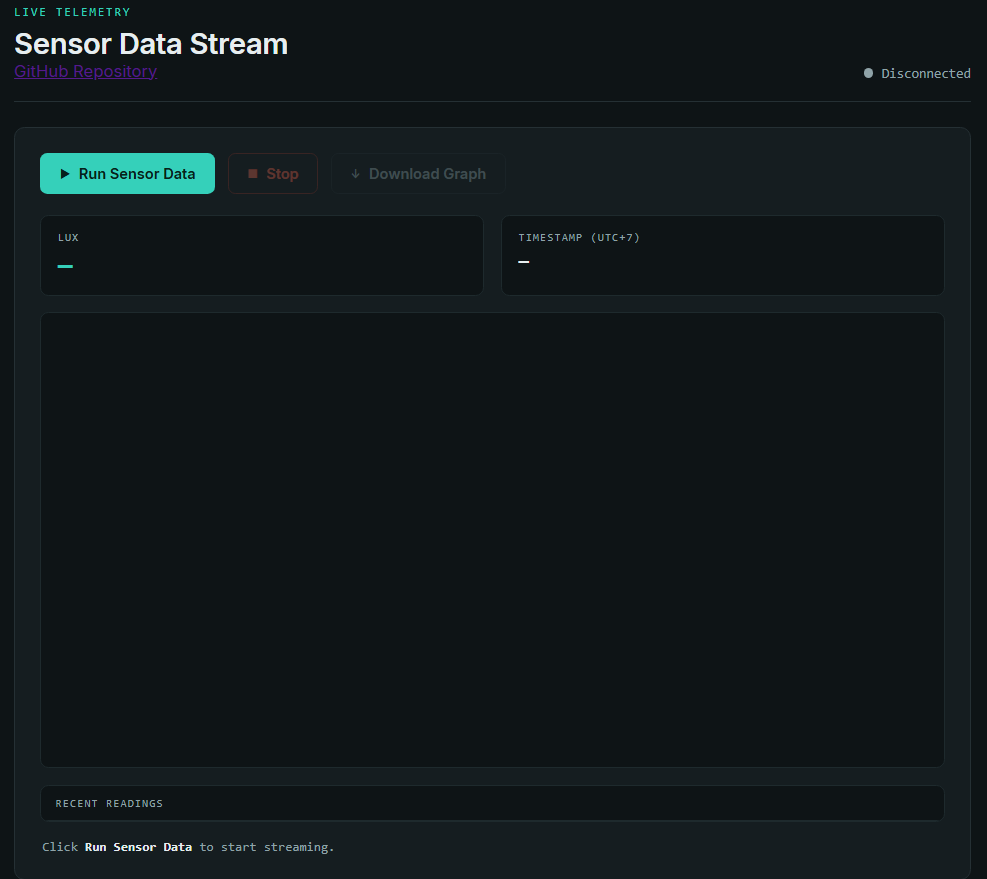
\includegraphics[width=0.9\textwidth]{Figures/gui.png}
    \caption{Web-based graphical user interface developed for real-time light monitoring.}
    \label{fig:gui}
\end{figure}


% ------------------------------------------------------------------------------------
\section{Software Implementation}
The implementation consists of four main components. The STM32 firmware communicates with the BH1750 sensor through the I\textsuperscript{2}C interface and periodically acquires illumination measurements. A Python application receives the transmitted data through the USB Virtual COM Port and converts them into a structured JSON format. The Node.js backend server validates the received messages and distributes them to connected web clients through WebSocket communication. Finally, the frontend application updates the graphical user interface and visualizes the measurements in real time.

% ------------------------------------------------------------------------------------
\subsection{STM32 Firmware}

The STM32 firmware is responsible for communicating with the BH1750 light sensor and acquiring illumination measurements periodically. The firmware is developed using the STM32 Hardware Abstraction Layer (HAL), which provides high-level functions for peripheral initialization and communication.\\[0.1em]

During system initialization, the I\textsuperscript{2}C peripheral is configured and the BH1750 sensor is placed into Continuous High Resolution Mode. This operating mode enables the sensor to perform continuous measurements without requiring repeated configuration commands after each conversion.\\[0.1em]

\begin{lstlisting}[language=C, caption={Main measurement loop of the STM32 firmware.}, label={lst:stm32_loop}]
BH1750_ReadData();                         // Read sensor measurement

raw = ((uint16_t)buffer[0] << 8) | buffer[1];
// Combine MSB and LSB into a 16-bit value

lux = raw / 1.2f;                          // Convert raw value to lux

int length = sprintf(uartBuffer, "%.2f\r\n", lux);
// Format the lux value as an ASCII string

HAL_UART_Transmit(&huart2,
                  (uint8_t *)uartBuffer,
                  length,
                  HAL_MAX_DELAY);
// Transmit the formatted string to the PC

HAL_Delay(1000);                           // Wait 1 second
\end{lstlisting}

\vspace{0.5em}

\autoref{lst:stm32_loop} presents the main execution loop of the STM32 firmware. First, the microcontroller reads the two-byte measurement from the BH1750 sensor through the I\textsuperscript{2}C interface. The received most significant byte (MSB) and least significant byte (LSB) are combined into a single 16-bit unsigned integer representing the raw sensor output. The firmware then converts this raw value into illumination (lux) using the conversion relationship introduced in Equation~\eqref{eq:lux_conversion}.\\[0.1em]

The calculated illumination value is formatted as an ASCII string with two decimal places using the \textit{\texttt{sprintf()}} function before being transmitted to the host computer via the UART interface. Finally, the firmware waits for one second before acquiring the next measurement, resulting in a sampling rate of approximately 1 Hz.

% ------------------------------------------------------------------------------------
\subsection{Python Serial Reader}

The Python Serial Reader serves as the communication bridge between the STM32 microcontroller and the backend server.The application is implemented using the \texttt{pySerial} library for serial communication and the \texttt{websocket-client} library for WebSocket communication.\\[0.1em]

The STM32 periodically transmits illumination measurements as ASCII strings terminated by a newline character. Upon receiving a serial packet, the Python application decodes the incoming bytes using UTF-8 encoding and converts the resulting string into a floating-point number. Invalid packets, decoding failures, or malformed numerical values are discarded to prevent corrupted data from propagating through the communication pipeline.\\[0.1em]

After validation, the illumination value is serialized using the \texttt{json.dumps()} function before being transmitted to the backend server through a persistent WebSocket connection.

\begin{lstlisting}[language=Python,
caption={Transmission of validated sensor data to the backend server.},
label={lst:python_ws}]
lux = ser.readline()                  # Read one UART packet
payload = into_json(lux)              # Validate and convert to float

if payload is not None: 
    json_output = json.dumps(payload) # Serialize into JSON format
    ws.send(json_output)              # Send to the server
\end{lstlisting}

\vspace{0.5em}

As shown in \autoref{lst:python_ws}, the application first reads one measurement from the serial interface and converts it into a floating-point value using the \texttt{into\_json()} function. This implementation keeps the Python application lightweight by delegating message formatting and client broadcasting to the backend server.

% ------------------------------------------------------------------------------------
\subsection{Backend Server}

The Backend server serves as the communication bridge between the Python Serial Reader and the web-based graphical user interface. It is responsible for hosting the frontend application, receiving illumination measurements from the Python client through a WebSocket connection, validating the received data, and forwarding the measurements to all connected browser clients.\\[0.1em]

The backend is implemented using the Express framework to provide HTTP services and the \texttt{ws} library to implement WebSocket communication. The Express server hosts the static frontend resources, including the HTML, CSS, and JavaScript files, while the WebSocket server enables real-time bidirectional communication between the backend and connected clients.\\[0.1em]

After successful validation, the illumination value is serialized and immediately broadcast to every browser currently connected to the WebSocket server.

\begin{lstlisting}[language=JavaScript,
caption={Validation and broadcasting of sensor measurements in the Node.js backend.},
label={lst:server_backend}]
lux = JSON.parse(data.toString());      // Parse received message

if (!Number.isFinite(Number(lux)) ||
    Number(lux) < 0) {
    return;                             // Ignore invalid data
}

const sensorMessage =
    JSON.stringify(Number(lux));        // Serialize measurement

for (const client of wss.clients) {
    if (client.readyState === WebSocket.OPEN) {
        client.send(sensorMessage);     // Broadcast to all browsers
    }
}
\end{lstlisting}

\vspace{0.5em}

\autoref{lst:server_backend} illustrates the core functionality of the Node.js backend. After receiving a message from the Python Serial Reader, the server parses the incoming data and verifies that it represents a valid non-negative numerical illumination value. The validated measurement is then serialized and broadcast to every browser currently connected to the WebSocket server. This approach enables multiple users to observe the same sensor measurements simultaneously while maintaining a simple and efficient communication architecture.


% ------------------------------------------------------------------------------------
\subsection{Web-Based Frontend}

As described in \hyperref[sec:web_gui]{Section~\ref*{sec:web_gui}, \textit{User Interface}}, the frontend establishes a WebSocket connection with the backend server, receives incoming sensor measurements, and updates the displayed information dynamically without requiring the webpage to be refreshed.\\[0.1em]

Upon loading the webpage, the JavaScript application creates a persistent WebSocket connection to the backend server. This communication channel enables the frontend to receive new illumination measurements immediately after they are broadcast by the backend server.\\[0.1em]

Whenever a new sensor measurement is received, the frontend parses the incoming message and updates the displayed illumination value.

\begin{lstlisting}[language=JavaScript,
caption={Processing incoming WebSocket messages in the frontend.},
label={lst:frontend_ws}]
ws.addEventListener("message", (event) => {

    let lux;

    try {
        lux = JSON.parse(event.data);     // Parse the received lux value
    }
    catch (err) {
        console.error("Received invalid JSON:", event.data);
        return;                           // Ignore malformed packets
    }

    if (typeof lux === "number") {
        appendPoint(new Date(), lux);     // Update the real-time graph
    }
    else {
        console.warn("Unhandled message type");
    }

});
\end{lstlisting}

\vspace{0.5em}

\autoref{lst:frontend_ws} illustrates the processing performed when a new WebSocket message is received by the frontend application. First, the received message is parsed into a numerical illumination value using the \texttt{JSON.parse()} function. If the received data are malformed, the packet is discarded to prevent invalid information from being displayed.\\[0.1em]

After successful parsing, the application verifies that the received value is of numerical type before updating the graphical visualization. The current local system time is recorded and associated with the received measurement, while the illumination value is appended to the Plotly \cite{plotly_js} time-series graph.

\begin{lstlisting}[language=JavaScript,
caption={Updating the real-time Plotly graph.},
label={lst:append_point}]
export function appendPoint(timestamp, value) {

    // Use the received timestamp or generate the current time
    const raw = timestamp !== undefined
        ? timestamp
        : new Date().toISOString();

    // Convert the timestamp to UTC+7 format
    const parts = getUTC7Parts(raw);
    const x = partsToPlotlyISOString(parts);

    // Store the new measurement locally
    state.xData.push(x);
    state.yData.push(value);

    // Append the new point to the existing Plotly graph
    Plotly.extendTraces(
        plotDiv,
        { x: [[x]], y: [[value]] },
        [0]
    );

    // Refresh the numerical reading panel
    updateReadingPanel(parts, value);
}
\end{lstlisting}

\vspace{0.5em}

\autoref{lst:append_point} illustrates the procedure used to update the graphical user interface whenever a new illumination measurement is received. First, the timestamp is converted into the local time zone (UTC+7) before being appended to the horizontal axis of the graph. The corresponding illumination value is then stored together with the timestamp.\\[0.1em]

The Plotly function \texttt{extendTraces()} appends the new data point to the existing graph without redrawing the entire figure, thereby enabling efficient real-time visualization. Finally, the numerical display panel is refreshed to present the latest lux value and acquisition time to the user.

% ------------------------------------------------------------------------------------
\section{Results and Discussion}

\subsection{Experimental Setup and Procedure}

The proposed monitoring system was evaluated under normal indoor lighting conditions. The experimental setup consisted of an STM32 microcontroller connected to a BH1750 digital light intensity sensor through the I\textsuperscript{2}C interface. The STM32 periodically measured the ambient illumination and transmitted the acquired values to a host computer via a USB Virtual COM Port.\\[0.1em]

To evaluate the proposed monitoring system, the following procedure was carried out.

\begin{enumerate}

    \item First, the Node.js backend server was started from a terminal using the command \texttt{node server.js}. This launched both the HTTP server and the WebSocket server, making the web application available on the local host.

    \begin{figure}[H]
        \centering
        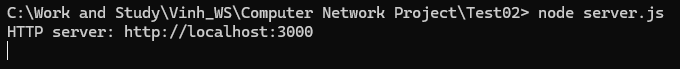
\includegraphics[width=\textwidth]{Figures/run_server.png}
        \caption{Starting the Node.js backend server.}
        \label{fig:run_server}
    \end{figure}

    \item Next, the Python Serial Reader was executed using the command \texttt{python read\_sensor.py}. The application established a serial connection with the STM32 through the USB Virtual COM Port, continuously received illumination measurements from the BH1750 sensor, and forwarded the validated measurements to the backend server through a WebSocket connection.

    \begin{figure}[H]
        \centering
        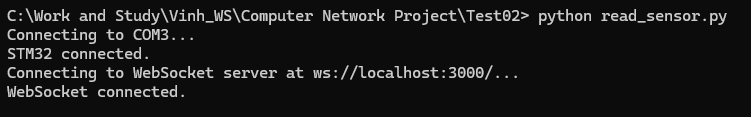
\includegraphics[width=\textwidth]{Figures/run_reading_sensor.png}
        \caption{Running the Python Serial Reader and establishing the WebSocket connection.}
        \label{fig:run_python}
    \end{figure}

    \item Finally, the local web server was exposed to external clients using \textbf{ngrok} \cite{ngrok_docs}, a globally distributed reverse proxy. The HTTP endpoint \texttt{http://localhost:3000} was tunneled through ngrok, generating a public URL that allowed remote users to access the web interface and receive real-time sensor measurements.

\end{enumerate}

    \begin{figure}[H]
        \centering
        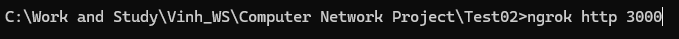
\includegraphics[width=0.9\textwidth]{Figures/ngrok_setup.png}\\[0.5em]
        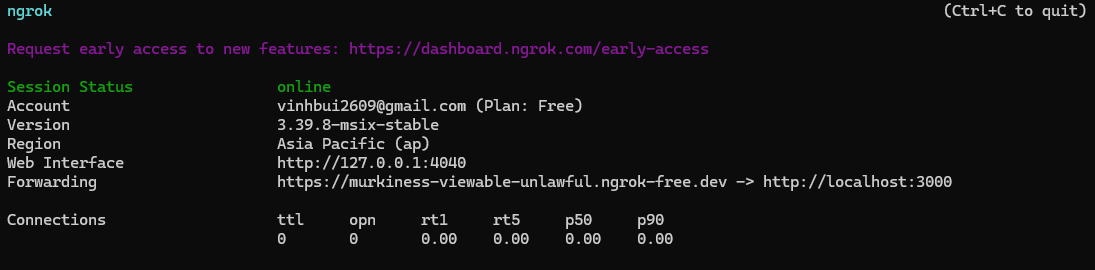
\includegraphics[width=0.9\textwidth]{Figures/ngrok_running.png}
        \caption{Publishing the local web server using ngrok.}
        \label{fig:run_ngrok}
    \end{figure}
    
   By exposing the local HTTP server through a secure public URL, remote users were able to access the graphical user interface from different devices while receiving the same real-time sensor measurements. This confirms that the proposed architecture can support Internet-based monitoring without requiring modifications to the application software.\\[0.1em]


\subsection{Real-Time Monitoring Results}
\begin{figure}[H]
    \centering
    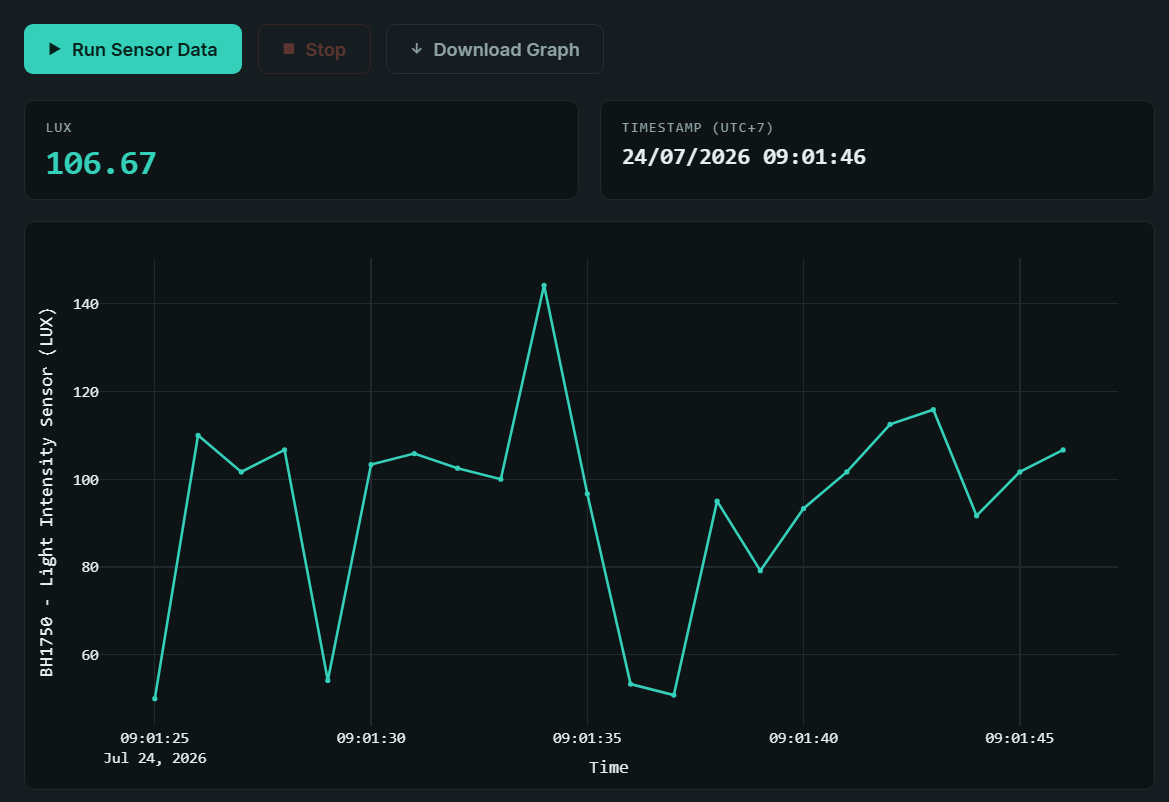
\includegraphics[width=\textwidth]{Figures/1.png}
    \caption{Main web-based graphical user interface during real-time monitoring.}
    \label{fig:1}
\end{figure}

\autoref{fig:1} illustrates the web interface during real-time monitoring. The upper information panel displays the latest illumination measurement acquired from the BH1750 sensor. The measured light intensity is presented in units of lux (lx) and is updated automatically whenever a new sensor reading is received from the backend server.\\[0.1em]

Alongside the measured lux value, the interface displays the timestamp corresponding to the latest received measurement. The timestamp is presented using the local time zone (UTC+7), allowing users to identify the exact time at which each measurement was recorded. Both the sensor value and timestamp are refreshed continuously, providing users with immediate feedback on the current lighting conditions.\\[0.1em]

The lower section of the interface presents a real-time line graph that visualizes the variation of light intensity over time. Each newly received measurement is appended to the graph immediately after arrival, enabling continuous monitoring of ambient illumination. This graphical representation allows users to observe both instantaneous changes and overall trends in the measured light intensity more effectively than numerical values alone.

\begin{figure}[H]
    \centering
    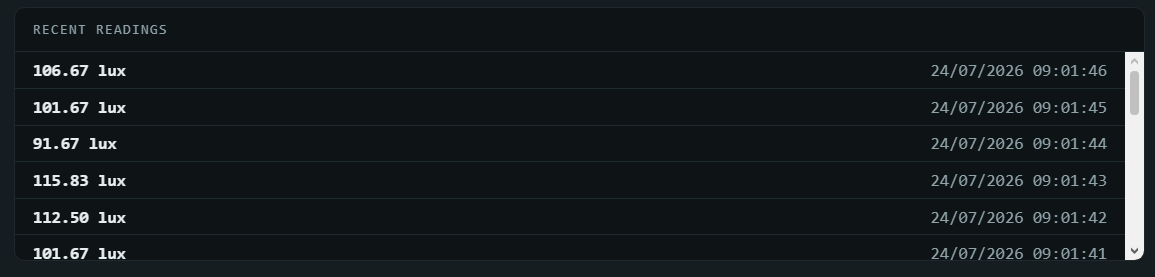
\includegraphics[width=\textwidth]{Figures/2.png}
    \caption{Recent sensor readings displayed in chronological order.}
    \label{fig:2}
\end{figure}

\autoref{fig:2} shows the recent readings panel of the web interface. Each entry contains the measured illumination value in lux together with the timestamp indicating when the measurement was acquired.\\[0.1em]

The table is updated dynamically as new sensor data arrive, with the most recent measurement displayed at the top of the list. This feature allows users to review previously recorded values without relying solely on the graphical visualization. The combination of numerical records and graphical trends improves the usability of the monitoring system by providing both precise measurements and an overview of changes in ambient light intensity.

%---------------------------------------------------------------------------
\section{Conclusion}

This project presented the design and implementation of a real-time light intensity monitoring system using the BH1750 digital light sensor, an STM32 microcontroller, and a web-based graphical user interface. The proposed system successfully integrates embedded hardware and modern web technologies to provide continuous monitoring of ambient illumination through a standard web browser.\\[0.1em]

The STM32 microcontroller periodically acquires illumination measurements from the BH1750 sensor via the I\textsuperscript{2}C interface and transmits the measured values to a host computer through a USB Virtual COM Port. A Python application receives the serial data, validates the measurements, and forwards them to a Node.js backend server using a WebSocket connection. The backend subsequently distributes the received measurements to connected web clients, where the frontend dynamically updates the numerical display and the Plotly time-series graph in real time.\\[0.1em]

Experimental results demonstrated that the complete communication pipeline operated reliably, enabling low-latency transmission of sensor measurements from the hardware to the web interface. The modular software architecture also proved effective by separating the embedded firmware, serial communication, backend processing, and frontend visualization into independent components, thereby simplifying development, testing, and future maintenance.

\newpage
    

\bibliographystyle{IEEEtran}
\bibliography{references}

% ---------------------------------------------------
\newpage
\section{ANNEX}
\subsection{read\_sensor.py}
    \begin{lstlisting}[language=Python]
import serial
import time
import json

import websocket

PORT = "COM3"
BAUD_RATE = 9600
TIMEOUT = 1
WS_URL = "ws://localhost:3000/"


def connect_serial():
    print(f"Connecting to {PORT}...")

    ser = serial.Serial(
        port=PORT,
        baudrate=BAUD_RATE,
        parity=serial.PARITY_NONE,
        stopbits=serial.STOPBITS_ONE,
        bytesize=serial.EIGHTBITS,
        timeout=TIMEOUT
    )

    print("STM32 connected.")
    return ser


def into_json(raw_bytes):
    try:
        text = raw_bytes.decode("utf-8").strip()

        if not text:
            return None

        value = float(text)
        return value

    except UnicodeDecodeError:
        print("WARNING: UTF-8 decoding failed.")
        return None

    except ValueError:
        print(f"WARNING: Invalid numeric value received: '{text}'")
        return None



def open_websocket():
    while True:
        try:
            print(f"Connecting to WebSocket server at {WS_URL}...")
            ws = websocket.create_connection(WS_URL, timeout=5)
            print("WebSocket connected.")
            return ws
        except (OSError, websocket.WebSocketException) as error:
            print(f"WebSocket connection failed: {error}")
            time.sleep(2)


def main():
    ser = None
    ws = None

    while True:
        try:
            if ser is None or not ser.is_open:
                ser = connect_serial()
            
            if ws is None or not ws.connected:
                ws = open_websocket()

            lux = ser.readline()
            payload = into_json(lux)

            if payload is not None:
                json_output = json.dumps(payload)
                ws.send(json_output)

        except serial.SerialException as error:
            print(f"Serial connection lost: {error}")
            if ser is not None:
                ser.close()
            ser = None
            time.sleep(2)

        except (websocket.WebSocketException, OSError) as error:
            print(f"WebSocket connection lost: {error}")
            if ws is not None:
                try:
                    ws.close()
                except Exception:   
                    pass
            ws = None
            time.sleep(2)

        except KeyboardInterrupt:
            if ser is not None and ser.is_open:
                ser.close()
            if ws is not None:
                ws.close()
            print("\nProgram stopped.")
            break


if __name__ == "__main__":
    main()

    \end{lstlisting}

\subsection{server.js}
    \begin{lstlisting}[language=JavaScript]
const express = require("express");
const path = require("path");
const http = require("http");
const WebSocket = require("ws");

const app = express();
const PORT = 3000;
const ROOT = __dirname;

app.use(express.static(path.join(ROOT, "public")));

app.get("/", (req, res) => {
  res.sendFile(path.join(ROOT, "public", "index.html"));
});

const server = http.createServer(app);
const wss = new WebSocket.Server({ server });

wss.on("connection", (socket, request) => {
  const host = request.headers.host || `localhost:${PORT}`;
  console.log("WebSocket connected");

  socket.on("message", (data) => {
  let lux;

  try {
    lux = JSON.parse(data.toString());
  } catch {
    return;
  }

  if (!Number.isFinite(Number(lux)) || Number(lux) < 0) {
    return;
  }

  const sensorMessage = JSON.stringify(Number(lux));

  console.log("Lux:", lux);

  for (const client of wss.clients) {
    if (client.readyState === WebSocket.OPEN) {
      client.send(sensorMessage);
    }
  }
  });

  socket.on("close", () => {
    console.log(`WebSocket disconnected: ${socket.role}`);
  });

  socket.on("error", (error) => {
    console.error("WebSocket error:", error.message);
  });
});

server.listen(PORT, () => {
  console.log(`HTTP server: http://localhost:${PORT}`);
});

    \end{lstlisting}

\subsection{home.js}
    \begin{lstlisting}[language=JavaScript]
// --- Imports -----------------------------------------------------------
import { runBtn, stopBtn, downloadBtn, downloadDropdown, downloadMenu } from "./home-DOM.js";
import { initPlot, downloadGraph } from "./home-plotly.js";
import { connectAndStart, stopStreaming } from "./home-WebSocket.js";

initPlot();

// --- Event wiring ------------------------------------------------------
runBtn.addEventListener("click", connectAndStart);
stopBtn.addEventListener("click", stopStreaming);

// --- Dropdown menu behavior --------------------------------------------
// Open menu
downloadBtn.addEventListener("click", (event) => {
  event.stopPropagation();
  downloadMenu.classList.toggle("is-open");
});

// Close menu
document.addEventListener("click", (event) => {
  if (!downloadDropdown.contains(event.target)) {
    downloadMenu.classList.remove("is-open");
  }
});

// Format Selected -> get format type from HTML
downloadMenu.querySelectorAll(".dropdown__item").forEach((item) => {
  item.addEventListener("click", () => {
    downloadMenu.classList.remove("is-open");
    downloadGraph(item.dataset.format);
  });
}); 
    \end{lstlisting}  

\subsection{home-WebSocket.js}
    \begin{lstlisting}[language=JavaScript]
// --- Imports -----------------------------------------------------------
import {
  runBtn,
  stopBtn,
  downloadBtn,
  statusEl,
  statusDot,
  statusLabel,
  hint,
  plotDiv,
  currentLuxEl,
  currentTimeEl,
  logListEl
} from "./home-DOM.js"

import {state, initPlot, appendPoint} from "./home-plotly.js"

// --- Configuration -----------------------------------------------------
// Matches server.js: http.createServer + WebSocket.Server on the same port.
const WS_URL = "ws://localhost:3000";

// --- UI state helpers ------------------------------------------------------
function setStatus(mode, label) {
  statusEl.classList.remove("is-live", "is-error");
  if (mode === "live") statusEl.classList.add("is-live");
  if (mode === "error") statusEl.classList.add("is-error");
  statusLabel.textContent = label;
}

function setStreamingUI(isStreaming) {
  state.streaming = isStreaming;
  runBtn.disabled = isStreaming;
  stopBtn.disabled = !isStreaming;
  hint.innerHTML = isStreaming
    ? "Streaming live sensor data&hellip; click <strong>Stop</strong> to end the session."
    : "Click <strong>Run Sensor Data</strong> to start streaming.";
}

// --- WebSocket handling ------------------------------------------------------
export function connectAndStart() {
  setStatus("connecting", "Connecting…");
  runBtn.disabled = true; // prevent double-clicks while connecting

  const ws = new WebSocket(WS_URL);
  state.ws = ws;

  ws.addEventListener("open", () => {
    setStatus("live", "Streaming");
    setStreamingUI(true);
    // Reset the graph for a fresh run
    state.xData = [];
    state.yData = [];
    initPlot();
    currentLuxEl.textContent = "\u2014";
    currentTimeEl.textContent = "\u2014";
    logListEl.innerHTML = "";
  });

  ws.addEventListener("message", (event) => {
    let lux;

    try {
      lux = JSON.parse(event.data);   // event.data is a JSON number, e.g. 123.45
    } catch (err) {
      console.error("Received invalid JSON:", event.data);
      return;
    }

    if (typeof lux === "number") {
      appendPoint(new Date(), lux);
    } else {
      console.warn("Unhandled message type:");
    }
  });

  ws.addEventListener("close", () => {
    setStatus("idle", "Disconnected");
    setStreamingUI(false);
    downloadBtn.disabled = state.xData.length === 0;
  });

  ws.addEventListener("error", (err) => {
    console.error("WebSocket error:", err);
    setStatus("error", "Connection error");
  });
}

export function stopStreaming() {
  if (state.ws && state.ws.readyState === WebSocket.OPEN) {
    state.ws.close();
  }
  setStreamingUI(false);
  setStatus("idle", "Disconnected");
  downloadBtn.disabled = state.xData.length === 0;
}
    \end{lstlisting} 

\subsection{home-DOM.js}
    \begin{lstlisting}[language=JavaScript]
// --- DOM references ------------------------------------------------------

export const runBtn = document.getElementById("runBtn");

export const stopBtn = document.getElementById("stopBtn");

export const downloadBtn = document.getElementById("downloadBtn");

export const downloadMenu = document.getElementById("downloadMenu");

export const downloadDropdown = document.getElementById("downloadDropdown");

export const statusEl = document.getElementById("status");

export const statusDot = document.getElementById("statusDot");

export const statusLabel = document.getElementById("statusLabel");

export const hint = document.getElementById("hint");

export const plotDiv = document.getElementById("plot");

export const currentLuxEl = document.getElementById("currentLux");

export const currentTimeEl = document.getElementById("currentTime");

export const logListEl = document.getElementById("logList");
    \end{lstlisting} 

\subsection{home-plotly.js}
    \begin{lstlisting}[language=JavaScript]
// --- Imports ---------------------------------------------------------------
import { getUTC7Parts, partsToPlotlyISOString, formatUTC7Display} from "./home-time_zone.js";
import {
  plotDiv,
  currentLuxEl,
  currentTimeEl,
  logListEl
} from "./home-DOM.js"

// --- Plotly setup ----------------------------------------------------------
const plotLayout = {
  paper_bgcolor: "transparent",
  plot_bgcolor: "transparent",
  font: { color: "#e7eef0", family: "IBM Plex Mono, monospace", size: 12 },
  margin: { l: 50, r: 20, t: 20, b: 40 },
  xaxis: { title: "Time", gridcolor: "#1e2a2d", zeroline: false },
  yaxis: { title: "BH1750 - Light Intensity Sensor (LUX)", gridcolor: "#1e2a2d", zeroline: false },
  showlegend: false,
};

const plotConfig = { responsive: true, displayModeBar: false };

// --- Local state (per tab/session) ---------------------------------------
export const state = {
  ws: null,
  streaming: false,
  xData: [],
  yData: [],
};

export function initPlot() {
  const trace = {
    x: [],
    y: [],
    mode: "lines+markers",
    type: "scatter",
    line: { color: "#35d0ba", width: 2 },
    marker: { size: 4, color: "#35d0ba" },
  };
  Plotly.newPlot(plotDiv, [trace], plotLayout, plotConfig);
}

// --- Graph and Panel updates ------------------------------------------------------
export function appendPoint(timestamp, value) {
  const raw = timestamp !== undefined ? timestamp : new Date().toISOString();
  const parts = getUTC7Parts(raw);
  const x = partsToPlotlyISOString(parts);

  state.xData.push(x);
  state.yData.push(value);

  Plotly.extendTraces(plotDiv, { x: [[x]], y: [[value]] }, [0]);

  // Keep only the most recent N points visible to avoid the graph
  // becoming unreadable during long streams. Adjust as needed.
  const MAX_VISIBLE = 200;
  if (state.xData.length > MAX_VISIBLE) {
    const excess = state.xData.length - MAX_VISIBLE;
    Plotly.relayout(plotDiv, {
      "xaxis.range": [state.xData[excess], x],
    });
  }

  updateReadingPanel(parts, value);
}

function updateReadingPanel(parts, value) {
  const formattedTime = formatUTC7Display(parts);

  currentLuxEl.textContent = value.toFixed(2);
  currentTimeEl.textContent = formattedTime;

  const row = document.createElement("div");
  row.className = "log__row";
  row.innerHTML = `<span class="log__lux">${value.toFixed(2)} lux</span><span>${formattedTime}</span>`;
  logListEl.prepend(row);

  // Cap the log so it doesn't grow unbounded during a long stream.
  const MAX_LOG_ROWS = 50;
  while (logListEl.children.length > MAX_LOG_ROWS) {
    logListEl.removeChild(logListEl.lastChild);
  }
}

// --- Graph export (SVG / PNG / JSON) ------------------

function buildExportLayout() {
  return {
    ...plotLayout,
    paper_bgcolor: "#ffffff",
    plot_bgcolor: "#ffffff",
    font: { ...plotLayout.font, color: "#111111" },
    xaxis: {
      ...plotLayout.xaxis,
      gridcolor: "#cccccc",
      zerolinecolor: "#cccccc",
      linecolor: "#111111",
      tickfont: { color: "#111111" },
    },
    yaxis: {
      ...plotLayout.yaxis,
      gridcolor: "#cccccc",
      zerolinecolor: "#cccccc",
      linecolor: "#111111",
      tickfont: { color: "#111111" },
    },
  };
}

async function downloadImageFormat(format) {
  const hiddenDiv = document.createElement("div");
  hiddenDiv.style.position = "fixed";
  hiddenDiv.style.top = "0";
  hiddenDiv.style.left = "-9999px";
  hiddenDiv.style.width = "900px";
  hiddenDiv.style.height = "500px";
  document.body.appendChild(hiddenDiv);
 
  try {
    await Plotly.newPlot(hiddenDiv, plotDiv.data, buildExportLayout(), {
      staticPlot: true,
    });
    await Plotly.downloadImage(hiddenDiv, {
      format,
      filename: "sensor-graph",
      width: 900,
      height: 500,
    });
  } finally {
    Plotly.purge(hiddenDiv);
    hiddenDiv.remove();
  }
}

function downloadJSON() {
  const exportObject = {
    data: plotDiv.data,
    layout: plotDiv.layout,
  };
  const blob = new Blob([JSON.stringify(exportObject, null, 2)], {
    type: "application/json",
  });
  triggerDownload(blob, "sensor-graph.json");
}

function triggerDownload(blob, filename) {
  const url = URL.createObjectURL(blob);
  const a = document.createElement("a");
  a.href = url;
  a.download = filename;
  document.body.appendChild(a);
  a.click();
  a.remove();
  URL.revokeObjectURL(url);
}

export function downloadGraph(format) {
  if (format === "json") {
    downloadJSON();
  } else {
    downloadImageFormat(format);
  }
}

    \end{lstlisting} 

\subsection{home-time\_zone.js}
    \begin{lstlisting}[language=JavaScript]
// --- Timezone handling (UTC+7) ------------------------------------------
const UTC7_PART_FORMATTER = new Intl.DateTimeFormat("en-US", {
  timeZone: "Asia/Ho_Chi_Minh",
  year: "numeric",
  month: "2-digit",
  day: "2-digit",
  hour: "2-digit",
  minute: "2-digit",
  second: "2-digit",
  hour12: false,
});

export function getUTC7Parts(timestamp) {
  const date = new Date(timestamp);
  const parts = UTC7_PART_FORMATTER.formatToParts(date).reduce((acc, p) => {
    acc[p.type] = p.value;
    return acc;
  }, {});
  if (parts.hour === "24") parts.hour = "00";
  return parts;
}

export function partsToPlotlyISOString(parts) {
  return `${parts.year}-${parts.month}-${parts.day}T${parts.hour}:${parts.minute}:${parts.second}.000Z`;
}

export function formatUTC7Display(parts) {
  return `${parts.day}/${parts.month}/${parts.year} ${parts.hour}:${parts.minute}:${parts.second}`;
}
    \end{lstlisting}

\subsection{index.html}
    \begin{lstlisting}[language=HTML]
<!DOCTYPE html>
<html lang="en">
<head>
  <meta charset="UTF-8" />
  <meta name="viewport" content="width=device-width, initial-scale=1.0" />
  <title>Sensor Data Stream</title>
  <link rel="stylesheet" href="style.css" />
</head>
<body>
  <div class="app">
    <header class="app__header">
      <div class="app__title">
        <span class="app__eyebrow">Live Telemetry</span>
        <h1>Sensor Data Stream</h1>
      </div>
      <div class="status" id="status">
        <span class="status__dot" id="statusDot"></span>
        <span class="status__label" id="statusLabel">Disconnected</span>
      </div>
    </header>

    <main class="app__main">
      <section class="panel">
        <div class="panel__controls">
          <button id="runBtn" class="btn btn--primary">
            <span class="btn__icon">&#9654;</span> Run Sensor Data
          </button>
          <button id="stopBtn" class="btn btn--danger" disabled>
            <span class="btn__icon">&#9632;</span> Stop
          </button>
          <div class="dropdown" id="downloadDropdown">
            <button id="downloadBtn" class="btn btn--ghost" disabled>
              <span class="btn__icon">&#8595;</span> Download Graph
            </button>
            <div class="dropdown__menu" id="downloadMenu">
              <button class="dropdown__item" data-format="png">PNG image</button>
              <button class="dropdown__item" data-format="svg">SVG</button>
              <button class="dropdown__item" data-format="json">JSON (raw data)</button>
            </div>
          </div>
        </div>

        <div class="reading">
          <div class="reading__block">
            <span class="reading__label">Lux</span>
            <span class="reading__value" id="currentLux">&mdash;</span>
          </div>
          <div class="reading__block">
            <span class="reading__label">Timestamp (UTC+7)</span>
            <span class="reading__value reading__value--time" id="currentTime">&mdash;</span>
          </div>
        </div>

        <div class="panel__graph">
          <div id="plot"></div>
        </div>

        <div class="log">
          <div class="log__header">Recent readings</div>
          <div class="log__list" id="logList"></div>
        </div>

        <p class="panel__hint" id="hint">
          Click <strong>Run Sensor Data</strong> to start streaming.
        </p>
      </section>
    </main>
  </div>

  <script src="https://cdn.plot.ly/plotly-2.32.0.min.js"></script>
  <script type = "module" src="home.js"></script>
</body>
</html>
    \end{lstlisting}

\subsection{style.css}
    \begin{lstlisting}[language=CSS]
:root {
  --bg: #0e1416;
  --panel: #151d20;
  --panel-border: #253034;
  --text: #e7eef0;
  --text-dim: #8fa3a8;
  --accent: #35d0ba;
  --accent-dim: #1f8f7e;
  --danger: #e0654f;
  --danger-dim: #7a3229;
  --grid: #1e2a2d;
  --mono: "IBM Plex Mono", "SFMono-Regular", Consolas, monospace;
  --sans: "Inter", -apple-system, BlinkMacSystemFont, "Segoe UI", sans-serif;
}

* { box-sizing: border-box; }

html, body {
  margin: 0;
  padding: 0;
  background: var(--bg);
  color: var(--text);
  font-family: var(--sans);
  min-height: 100vh;
}

.app {
  max-width: 960px;
  margin: 0 auto;
  padding: 32px 20px 60px;
}

.app__header {
  display: flex;
  justify-content: space-between;
  align-items: flex-end;
  border-bottom: 1px solid var(--panel-border);
  padding-bottom: 20px;
  margin-bottom: 24px;
  flex-wrap: wrap;
  gap: 12px;
}

.app__eyebrow {
  display: block;
  font-family: var(--mono);
  font-size: 12px;
  letter-spacing: 0.12em;
  text-transform: uppercase;
  color: var(--accent);
  margin-bottom: 6px;
}

.app__title h1 {
  margin: 0;
  font-size: 28px;
  font-weight: 600;
  letter-spacing: -0.01em;
}

.status {
  display: flex;
  align-items: center;
  gap: 8px;
  font-family: var(--mono);
  font-size: 13px;
  color: var(--text-dim);
}

.status__dot {
  width: 9px;
  height: 9px;
  border-radius: 50%;
  background: var(--text-dim);
  transition: background 0.2s ease, box-shadow 0.2s ease;
}

.status.is-live .status__dot {
  background: var(--accent);
  box-shadow: 0 0 8px var(--accent);
  animation: pulse 1.4s ease-in-out infinite;
}

.status.is-error .status__dot {
  background: var(--danger);
  box-shadow: 0 0 8px var(--danger);
}

@keyframes pulse {
  0%, 100% { opacity: 1; }
  50% { opacity: 0.4; }
}

.panel {
  background: var(--panel);
  border: 1px solid var(--panel-border);
  border-radius: 10px;
  padding: 24px;
}

.panel__controls {
  display: flex;
  gap: 12px;
  flex-wrap: wrap;
  margin-bottom: 20px;
}

.dropdown {
  position: relative;
}

.dropdown__menu {
  display: none;
  position: absolute;
  top: calc(100% + 6px);
  left: 0;
  min-width: 180px;
  background: var(--panel);
  border: 1px solid var(--panel-border);
  border-radius: 8px;
  padding: 6px;
  box-shadow: 0 8px 24px rgba(0, 0, 0, 0.4);
  z-index: 10;
}

.dropdown__menu.is-open {
  display: flex;
  flex-direction: column;
  gap: 2px;
}

.dropdown__item {
  background: transparent;
  border: none;
  color: var(--text);
  font-family: var(--sans);
  font-size: 13.5px;
  text-align: left;
  padding: 8px 10px;
  border-radius: 5px;
  cursor: pointer;
}

.dropdown__item:hover {
  background: rgba(255, 255, 255, 0.06);
  color: var(--accent);
}

.btn {
  display: inline-flex;
  align-items: center;
  gap: 8px;
  padding: 10px 18px;
  font-family: var(--sans);
  font-size: 14px;
  font-weight: 600;
  border-radius: 7px;
  border: 1px solid transparent;
  cursor: pointer;
  transition: transform 0.08s ease, opacity 0.15s ease, background 0.15s ease;
}

.btn:active:not(:disabled) { transform: translateY(1px); }

.btn:disabled {
  opacity: 0.35;
  cursor: not-allowed;
}

.btn__icon { font-size: 11px; }

.btn--primary {
  background: var(--accent);
  color: #06201b;
}
.btn--primary:hover:not(:disabled) { background: #4ee0cb; }

.btn--danger {
  background: transparent;
  color: var(--danger);
  border-color: var(--danger-dim);
}
.btn--danger:hover:not(:disabled) {
  background: rgba(224, 101, 79, 0.1);
}

.btn--ghost {
  background: transparent;
  color: var(--text-dim);
  border-color: var(--panel-border);
}
.btn--ghost:hover:not(:disabled) {
  color: var(--text);
  border-color: var(--text-dim);
}

.panel__graph {
  background: var(--bg);
  border: 1px solid var(--grid);
  border-radius: 8px;
  padding: 8px;
}

.reading {
  display: flex;
  gap: 16px;
  margin-bottom: 16px;
  flex-wrap: wrap;
}

.reading__block {
  flex: 1;
  min-width: 180px;
  background: var(--bg);
  border: 1px solid var(--grid);
  border-radius: 8px;
  padding: 14px 16px;
}

.reading__label {
  display: block;
  font-family: var(--mono);
  font-size: 11px;
  letter-spacing: 0.08em;
  text-transform: uppercase;
  color: var(--text-dim);
  margin-bottom: 6px;
}

.reading__value {
  display: block;
  font-family: var(--mono);
  font-size: 26px;
  font-weight: 600;
  color: var(--accent);
  line-height: 1.1;
}

.reading__value--time {
  font-size: 18px;
  color: var(--text);
}

.log {
  margin-top: 16px;
  background: var(--bg);
  border: 1px solid var(--grid);
  border-radius: 8px;
  overflow: hidden;
}

.log__header {
  font-family: var(--mono);
  font-size: 11px;
  letter-spacing: 0.08em;
  text-transform: uppercase;
  color: var(--text-dim);
  padding: 10px 14px;
  border-bottom: 1px solid var(--grid);
}

.log__list {
  max-height: 160px;
  overflow-y: auto;
  font-family: var(--mono);
  font-size: 13px;
}

.log__row {
  display: flex;
  justify-content: space-between;
  padding: 6px 14px;
  border-bottom: 1px solid var(--grid);
  color: var(--text-dim);
}

.log__row:last-child {
  border-bottom: none;
}

.log__row .log__lux {
  color: var(--text);
  font-weight: 600;
}

#plot {
  width: 100%;
  height: 420px;
}

.panel__hint {
  margin: 16px 2px 0;
  font-family: var(--mono);
  font-size: 12.5px;
  color: var(--text-dim);
}

.panel__hint strong {
  color: var(--text);
  font-weight: 600;
}

@media (max-width: 600px) {
  .app__header { flex-direction: column; align-items: flex-start; }
  .panel__controls { flex-direction: column; }
  .btn { width: 100%; justify-content: center; }
  .dropdown { width: 100%; }
  .dropdown__menu { left: 0; right: 0; min-width: unset; }
  #plot { height: 320px; }
}
    \end{lstlisting}  

\subsection{BH1750.h}
    \begin{lstlisting}[language=C]
#ifndef BH1750_H_
#define BH1750_H_

#include <stdint.h>

/* Macro Command */
// Slave address
#define ADDR_HIGH_ADDRESS_WRITE 	(0xB8 + 0)
#define ADDR_HIGH_ADDRESS_READ 		(0xB8 + 1)
#define ADDR_LOW_ADDRESS_WRITE		(0x46 + 0)
#define ADDR_LOW_ADDRESS_READ 		(0x46 + 1)


// Commands table
#define BH1750_POWER_DOWN			0x00
#define BH1750_POWER_ON				0x01
#define BH1750_RESET				0x07
#define BH1750_CON_H_RES_MODE		0x10
#define BH1750_CON_H_RES_MODE2		0x11
#define BH1750_CON_L_RES_MODE		0x13
#define BH1750_ONE_H_RES_MODE		0x20
#define BH1750_ONE_H_RES_MODE2		0x21
#define BH1750_ONE_L_RES_MODE		0x23
#define BH1750_CHANGE_HIGH_MT		0x08	//01000_XXX
#define BH1750_CHANGE_LOW_MT		0x03	//011_XXXXX

// Sending data
#define POW_2_OF_15 	32768
#define POW_2_OF_9 		512
#define POW_2_OF_8		256
#define POW_2_OF_7 		128
#define POW_2_OF_4 		16


/* Function declaration */
void BH1750_ContinuousMode();
void BH1750_SendCommand(uint8_t cmd);
void BH1750_ReadData();


#endif
    \end{lstlisting} 

\subsection{BH1750.c}
    \begin{lstlisting}[language=C]
#include "BH1750.h"
#include "i2c.h"

extern uint8_t buffer[2];

// MODE pin -> LOW = Continuous Mode
void BH1750_ContinuousMode()
{
	 HAL_GPIO_WritePin(BH1750_MODE_GPIO_Port, BH1750_MODE_Pin, GPIO_PIN_RESET);
}


void BH1750_SendCommand(uint8_t cmd)
{
	HAL_I2C_Master_Transmit(&hi2c1, ADDR_LOW_ADDRESS_WRITE, &cmd, 1, HAL_MAX_DELAY);
}


void BH1750_ReadData()
{
    HAL_I2C_Master_Receive(&hi2c1, ADDR_LOW_ADDRESS_READ, buffer, 2, HAL_MAX_DELAY);
}
    \end{lstlisting} 

\subsection{main.c}
    \begin{lstlisting}[language=C]
/* USER CODE BEGIN Header */
/**
  ******************************************************************************
  * @file           : main.c
  * @brief          : Main program body
  ******************************************************************************
  * @attention
  *
  * Copyright (c) 2024 STMicroelectronics.
  * All rights reserved.
  *
  * This software is licensed under terms that can be found in the LICENSE file
  * in the root directory of this software component.
  * If no LICENSE file comes with this software, it is provided AS-IS.
  *
  ******************************************************************************
  */
/* USER CODE END Header */
/* Includes ------------------------------------------------------------------*/
#include "main.h"
#include "i2c.h"
#include "usart.h"
#include "gpio.h"

/* Private includes ----------------------------------------------------------*/
/* USER CODE BEGIN Includes */
#include "BH1750.h"
#include "usart.h"
#include <stdio.h>
/* USER CODE END Includes */

/* Private typedef -----------------------------------------------------------*/
/* USER CODE BEGIN PTD */

/* USER CODE END PTD */

/* Private define ------------------------------------------------------------*/
/* USER CODE BEGIN PD */

/* USER CODE END PD */

/* Private macro -------------------------------------------------------------*/
/* USER CODE BEGIN PM */

/* USER CODE END PM */

/* Private variables ---------------------------------------------------------*/

/* USER CODE BEGIN PV */

// Buffer used to receive the two-byte light measurement from the BH1750
uint8_t buffer[2] = {0};

// Raw 16-bit sensor output
uint16_t raw = 0;

float lux = 0.0f;
char uartBuffer[64];

/* USER CODE END PV */

/* Private function prototypes -----------------------------------------------*/
void SystemClock_Config(void);
/* USER CODE BEGIN PFP */

/* USER CODE END PFP */

/* Private user code ---------------------------------------------------------*/
/* USER CODE BEGIN 0 */

/* USER CODE END 0 */

/**
  * @brief  The application entry point.
  * @retval int
  */
int main(void)
{

  /* USER CODE BEGIN 1 */

  /* USER CODE END 1 */

  /* MCU Configuration--------------------------------------------------------*/

  /* Reset of all peripherals, Initializes the Flash interface and the Systick. */
  HAL_Init();

  /* USER CODE BEGIN Init */

  /* USER CODE END Init */

  /* Configure the system clock */
  SystemClock_Config();

  /* USER CODE BEGIN SysInit */

  /* USER CODE END SysInit */

  /* Initialize all configured peripherals */
  MX_GPIO_Init();
  MX_I2C1_Init();
  MX_USART2_UART_Init();
  /* USER CODE BEGIN 2 */

  // Setup Reading Mode as Continuous
  BH1750_ContinuousMode();

  // Power on the sensor
  BH1750_SendCommand(BH1750_POWER_ON);

  // Clear previous measurement data
  BH1750_SendCommand(BH1750_RESET);

  // Start continuous High Resolution measurement mode
  BH1750_SendCommand(BH1750_CON_H_RES_MODE);


  /* USER CODE END 2 */

  /* Infinite loop */
  /* USER CODE BEGIN WHILE */
  while (1)
  {
	  // Read two bytes from BH1750
	  BH1750_ReadData();

	  /*---------------------------------------------------------
	   * Combine MSB and LSB into one 16-bit value
	   *
	   * buffer[0] = High byte
	   * buffer[1] = Low byte
	   *--------------------------------------------------------*/
	  raw = ((uint16_t)buffer[0] << 8) | buffer[1];

	  /*---------------------------------------------------------
	   * Convert raw measurement into Lux
	   *
	   * According to BH1750 datasheet:
	   *      Lux = Raw / 1.2
	   *--------------------------------------------------------*/
	  lux = raw / 1.2f;

	  int length = sprintf(uartBuffer, "%.2f\r\n", lux);

	  HAL_UART_Transmit(&huart2, (uint8_t *)uartBuffer, length, HAL_MAX_DELAY);

	  /* Wait before requesting another measurement */
	  HAL_Delay(1000);

    /* USER CODE END WHILE */

    /* USER CODE BEGIN 3 */
  }
  /* USER CODE END 3 */
}

/**
  * @brief System Clock Configuration
  * @retval None
  */
void SystemClock_Config(void)
{
  RCC_OscInitTypeDef RCC_OscInitStruct = {0};
  RCC_ClkInitTypeDef RCC_ClkInitStruct = {0};

  /** Configure the main internal regulator output voltage
  */
  __HAL_RCC_PWR_CLK_ENABLE();
  __HAL_PWR_VOLTAGESCALING_CONFIG(PWR_REGULATOR_VOLTAGE_SCALE1);

  /** Initializes the RCC Oscillators according to the specified parameters
  * in the RCC_OscInitTypeDef structure.
  */
  RCC_OscInitStruct.OscillatorType = RCC_OSCILLATORTYPE_HSI;
  RCC_OscInitStruct.HSIState = RCC_HSI_ON;
  RCC_OscInitStruct.HSICalibrationValue = RCC_HSICALIBRATION_DEFAULT;
  RCC_OscInitStruct.PLL.PLLState = RCC_PLL_NONE;
  if (HAL_RCC_OscConfig(&RCC_OscInitStruct) != HAL_OK)
  {
    Error_Handler();
  }

  /** Initializes the CPU, AHB and APB buses clocks
  */
  RCC_ClkInitStruct.ClockType = RCC_CLOCKTYPE_HCLK|RCC_CLOCKTYPE_SYSCLK
                              |RCC_CLOCKTYPE_PCLK1|RCC_CLOCKTYPE_PCLK2;
  RCC_ClkInitStruct.SYSCLKSource = RCC_SYSCLKSOURCE_HSI;
  RCC_ClkInitStruct.AHBCLKDivider = RCC_SYSCLK_DIV1;
  RCC_ClkInitStruct.APB1CLKDivider = RCC_HCLK_DIV1;
  RCC_ClkInitStruct.APB2CLKDivider = RCC_HCLK_DIV1;

  if (HAL_RCC_ClockConfig(&RCC_ClkInitStruct, FLASH_LATENCY_0) != HAL_OK)
  {
    Error_Handler();
  }
}

/* USER CODE BEGIN 4 */

/* USER CODE END 4 */

/**
  * @brief  This function is executed in case of error occurrence.
  * @retval None
  */
void Error_Handler(void)
{
  /* USER CODE BEGIN Error_Handler_Debug */
  /* User can add his own implementation to report the HAL error return state */
  __disable_irq();
  while (1)
  {
  }
  /* USER CODE END Error_Handler_Debug */
}
#ifdef USE_FULL_ASSERT
/**
  * @brief  Reports the name of the source file and the source line number
  *         where the assert_param error has occurred.
  * @param  file: pointer to the source file name
  * @param  line: assert_param error line source number
  * @retval None
  */
void assert_failed(uint8_t *file, uint32_t line)
{
  /* USER CODE BEGIN 6 */
  /* User can add his own implementation to report the file name and line number,
     ex: printf("Wrong parameters value: file %s on line %d\r\n", file, line) */
  /* USER CODE END 6 */
}
#endif /* USE_FULL_ASSERT */
    \end{lstlisting} 

\end{document}


